\documentclass{article}
\usepackage[de]{ukon-infie}
\usepackage[utf8]{inputenc}
\usepackage{algorithm2e}
\usepackage{amsmath}
\usepackage{graphicx}
% kann de oder en sein
% kann bubble break, topexercise sein

\Names{Jonas Probst, Simon Giebenhain}
\Lecture[AnaVis]{Analyse und Visualisierung von Informationen}
\Term{WS 2017/18}

\begin{document}
    \begin{ukon-infie}[22.11.17]{4}

        \begin{exercise}[p=11]{Perceptron implementation of logical functions}
        The bias is always zero.
        
        	\question{}
        	{ $w_1 = 1$ and $w_2 = 1$. The threshold is $2$\\
        	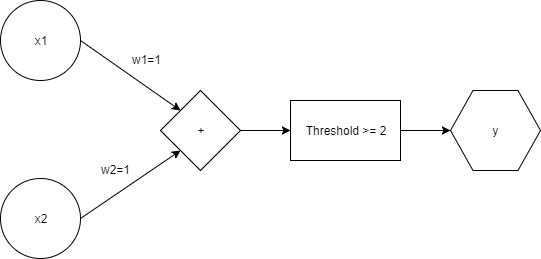
\includegraphics[scale=0.5]{A1a.png}} 
\begin{tabular}{|l|l|l|l|}
\hline
\textbf{x1} & \textbf{x2} & \textbf{+} & \textbf{y} \\ \hline
0           & 0           & 0          & 0          \\ \hline
1           & 0           & 1          & 0          \\ \hline
0           & 1           & 1          & 0          \\ \hline
1           & 1           & 2          & 1          \\ \hline
\end{tabular}

        	\question{}
        	{$w_1 = 1$ and $w_2 = 1$. The threshold is $1$\\
        	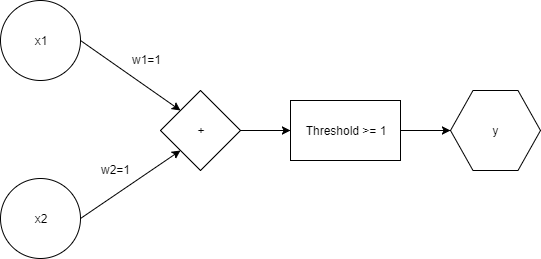
\includegraphics[scale=0.5]{A1b.png}
\begin{tabular}{|l|l|l|l|}
\hline
\textbf{x1} & \textbf{x2} & \textbf{+} & \textbf{y} \\ \hline
0           & 0           & 0          & 0          \\ \hline
1           & 0           & 1          & 1          \\ \hline
0           & 1           & 1          & 1          \\ \hline
1           & 1           & 2          & 1          \\ \hline
\end{tabular}
}
        	\question{}
        	{$w = -1$ and the threshold is $0$\\
        	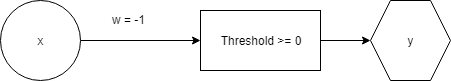
\includegraphics[scale=0.5]{A1c.png}
\begin{tabular}{|l|l|}
\hline
\textbf{x} & \textbf{y} \\ \hline
0          & 1          \\ \hline
1          & 0          \\ \hline
\end{tabular}
}
        	\question{}
        	{
        	The single-layer perceptron can only create a linear decision boundary. As illustrated below, one cannot draw a linea decision boundary, in order to classify the XOR correctly.\\
        	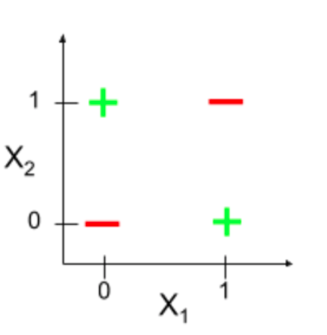
\includegraphics[scale=0.5]{perceptron_XOR}
        	}
		
		\end{exercise}
		
		\begin{exercise}[p=4]{Perceptron vs. SVM}
		An SVM tries to find an optimal solution by maximizing the margin. A Perceptron just tries to find any solution, so the seperating line can be closer to either class. So they could but likely won't find the same solution and hence not classify all grey points the same. A SVM would probably draw something like the green line, a perceptron can draw one of the yellow lines for example.\\
		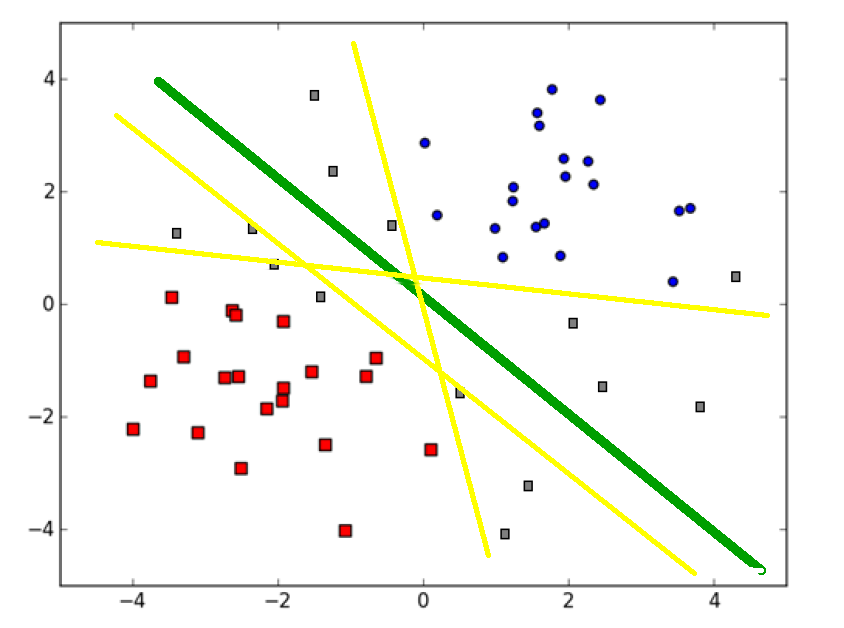
\includegraphics[scale=0.5]{points.png}
		
		\end{exercise}
		
		\begin{exercise}[p=2]{Sigmoid function}
			The major benefit of the sigmoid functions is that it is easily differentiable. Using the rule for differentiating fractions one finds:\\
			$sigmoid(x)' = sigmoid(x)(1- sigmoid(x))$.\\
			This property is especially important in algorithms which rely on the computing derivatives of the activation functions, like the Backpropagation algorithm.
		\end{exercise}
		
		


		\begin{exercise}[p=7+2]{Practical exercise}
		
		\question{}{
		The code below constructs 5 neural networks with 4 neurons in the hidden layer. The networks are trained for 3 cycles on the iris data set.\\
		The initialization of the weights is random. Because 3 training cycles are not sufficient to alter and improve the weights much, the performance of networks is very different and rather bad. However one of our networks was quiet lucky with the random initialization and was already proficient in calssifying irisis of the first two classes. Most of the other networks predicted wrong and the probabolities for the different calsses were similar.\\
		In contrast if one traines the networks for 100 iterations the performance is much better. The value(training error) often lies around 5. In comparison, after 3 iterations the value was around 160.
		}
		\begin{verbatim}
		library(nnet)
		nn1 <- nnet(Species~., data=iris, size=4, maxit=3)
		nn2 <- nnet(Species~., data=iris, size=4, maxit=3)
		nn3 <- nnet(Species~., data=iris, size=4, maxit=3)
		nn4 <- nnet(Species~., data=iris, size=4, maxit=3)
		nn5 <- nnet(Species~., data=iris, size=4, maxit=3)
		predict(nn1, newdata=iris)
		predict(nn2, newdata=iris)
		predict(nn3, newdata=iris)
		predict(nn4, newdata=iris)
		predict(nn5, newdata=iris)
		\end{verbatim}
		
		\question{}{
		When only changing one of the 2 parameters, like in the code below, it is much more beneficial to increase the numer of iterations, instead of the number of neurons in the hidden layer. When I ran the code below, I got an error of roughly 5 for nn\_iter and 200 for nn\_big.\\
		Furthermore one can see from the bonus exercise, that the iteration parameter has a bigger influence on the performence. However one has to note, that with a very small hidden layer(let's say below 4) the performance deteriorates.
		}
		\begin{verbatim}
		nn_iter <- nnet(Species~., data=iris, size=4, maxit=100)
		nn_big <- nnet(Species~., data=iris, size=100, maxit=3)
		\end{verbatim}
		
		\question{}
		{
		Note: For some reason x- and y-axes are switched in the plotting. That means that in the plot x represents the iterations and y the size.\\
		I have described ther influence of iterations and size above.\\
		Here are the plots of all combinations of size 1 to 20 and maxit 1 to 20. The z axis reprenstens the value/error.\\
		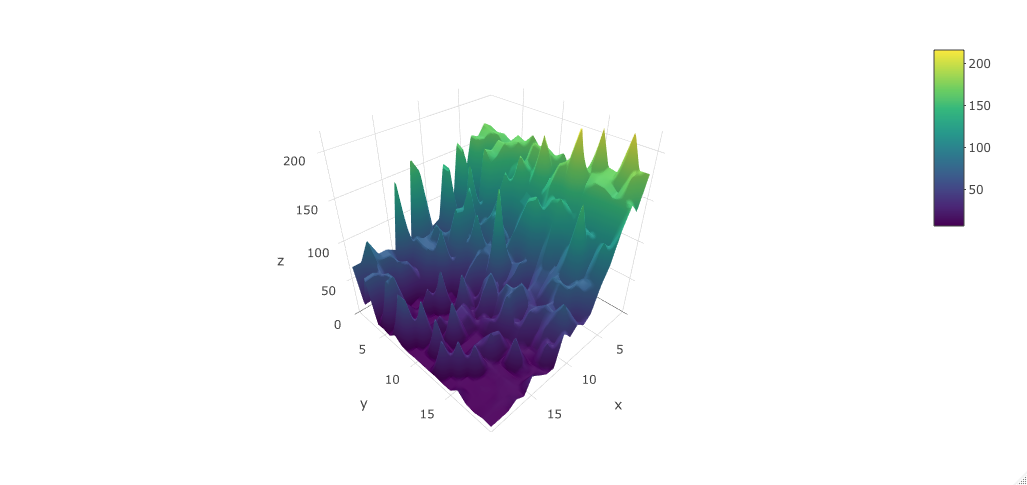
\includegraphics[scale=0.5]{Rplot_nn_iter_size}
		
		Espacially when one looks at the influence of the x-axis(representing the number of itersations), one observes, that this parameter is the major influence in this scenario. \\
		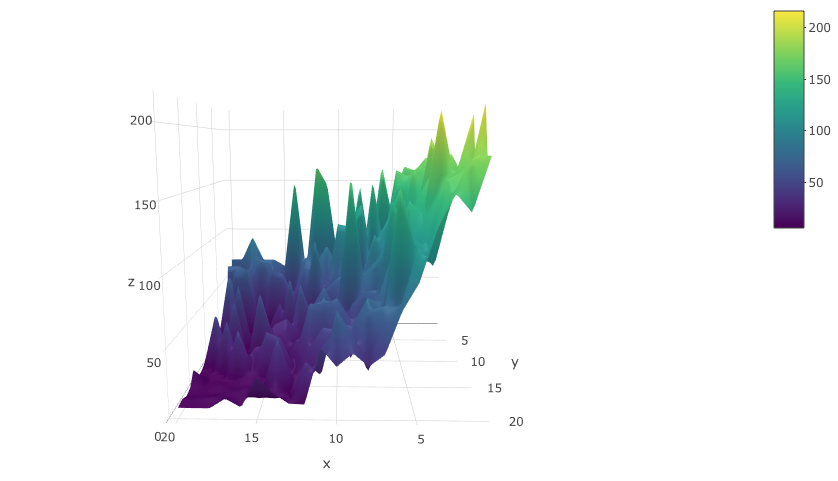
\includegraphics[scale=0.5]{Rplot_nn_iter_size_x}

		}
		\begin{verbatim}
		library(plotly)
		library(nnet)
		z <- array(1:400, dim=c(20,20))
		for (i in 1:20) {
    		for (j in 1:20) {
        		nn <- nnet(Species~., data=iris, size=i, maxit=j)
        		z[i,j] <- nn[["value"]]
    		}
		}
		plot_ly(x=1:20, y=1:20, z=z, type="surface")
		\end{verbatim}

		\end{exercise}
		
		
\end{ukon-infie}
\end{document}
